\documentclass[12pt,a4paper]{report}

% Encodage et langue
\usepackage[utf8]{inputenc}
\usepackage[T1]{fontenc}
\usepackage[french]{babel}
\usepackage{lmodern}

% Mise en page
\usepackage[a4paper,margin=1.5cm]{geometry}
\usepackage{setspace}
\onehalfspacing

% Graphiques et images
\usepackage{graphicx}
\usepackage{float}
\usepackage[table]{xcolor}

% Personnalisation des titres
\usepackage{titlesec}
\renewcommand{\thechapter}{\Roman{chapter}}
\titleformat{\chapter}[block]{\Huge\bfseries}{\Roman{chapter} --}{10pt}{}

% Table des matières
\usepackage{tocloft}
\renewcommand{\cftchapleader}{\cftdotfill{\cftdotsep}}
\renewcommand{\cftsecleader}{\cftdotfill{\cftdotsep}}
\renewcommand{\cftsubsecleader}{\cftdotfill{\cftdotsep}}

% Listes
\usepackage{enumitem}

% Tableaux longs
\usepackage{longtable}
\usepackage{tabularx}

% Symboles mathématiques (pour \square dans les tableaux)
\usepackage{amssymb}

% Hyperliens
\usepackage{hyperref}

\begin{document}

% ------------------------------------------------------------------
% Page de garde -- reconstructed from the original cover layout.
% Uses minipage for the header block (logo + institution text),
% a horizontal rule, centred titles, a framed project name,
% and bottom-aligned author / supervisor / year information.
% ------------------------------------------------------------------
\begin{titlepage}
    \newgeometry{left=2.5cm,right=2.5cm,top=2cm,bottom=2cm}

    % --- Header: logo (left) + institution info (right) ---
    \noindent
    \begin{minipage}[t]{0.30\textwidth}
        \vspace{0pt}
        % Replace "tekup_logo.png" with the actual logo file path.
        % 
\includegraphics[width=\linewidth]{tekup_logo.png}
        \raggedright
        {\fontsize{16}{18}\selectfont\bfseries \textcolor{blue!80!black}{TEK-UP}}\\[2pt]
        {\small\itshape University}
    \end{minipage}%
    \hfill
    \begin{minipage}[t]{0.60\textwidth}
        \vspace{0pt}
        \raggedleft
        {\normalsize\textbf{REPUBLIQUE TUNISIENNE}}\\[2pt]
        {\small Minist\`ere de l'Enseignement Sup\'erieur}\\
        {\small et de la Recherche Scientifique}\\[4pt]
        {\small\textbf{\'ECOLE SUP\'ERIEURE PRIV\'EE}}\\
        {\small\textbf{DE TECHNOLOGIES \& ING\'ENIERIE}}
    \end{minipage}

    \vspace{0.8cm}

    % --- Horizontal rule ---
    \noindent\rule{\textwidth}{0.8pt}

    \vspace{2.0cm}

    % --- Report type ---
    \begin{center}
        {\LARGE\bfseries\itshape Rapport de projet D\'eveloppement}
    \end{center}

    \vspace{1.8cm}

    % --- Programme title ---
    \begin{center}
        {\Large\bfseries\itshape Cycle de Formation des Ing\'enieurs\\[4pt]
        en Informatique}
    \end{center}

    \vspace{1.5cm}

    % --- Boxed project name ---
    \begin{center}
        \fbox{\parbox{0.55\textwidth}{\centering\large\bfseries\itshape SaveSafe Wallet SSW}}
    \end{center}

    \vfill

    % --- Authors, supervisor, academic year ---
    \begin{center}
        {\large\bfseries\itshape R\'ealis\'e par :}\\[6pt]
        {\normalsize AMOR Houssem, KHEDHIRI Montaha,}\\[2pt]
        {\normalsize BEN SLIMA Wissem, BAHROUNI Seif}\\[18pt]

        {\large\bfseries\itshape Encadr\'e par :}\\[6pt]
        {\normalsize Ines AGREBI}\\[18pt]

        {\large\bfseries\itshape Ann\'ee Universitaire :} {\normalsize 2025-2026}
    \end{center}

    \vspace{1cm}
    \restoregeometry
\end{titlepage}

\tableofcontents
\listoffigures
\listoftables
\newpage

% ==========================
% Introduction Générale (non numérotée)
% ==========================
\chapter*{Introduction Générale}
\addcontentsline{toc}{chapter}{Introduction Générale}

Le présent rapport s'inscrit dans le cadre du module \textit{Projet de Développement} du cycle de formation des ingénieurs en informatique à l'École Supérieure Privée de Technologies et d'Ingénierie (TEK-UP), pour l'année universitaire 2025-2026.

Le projet \textbf{SaveSafe Wallet (SSW)} consiste à concevoir et développer une plateforme web bancaire sécurisée, intégrant un portefeuille numérique (\textit{wallet}) et un système anti-piratage propulsé par l'Intelligence Artificielle. L'objectif est de fournir aux utilisateurs finaux une expérience bancaire moderne, tout en offrant aux administrateurs un tableau de bord de sécurité en temps réel alimenté par des modèles d'IA open-source (Ollama, Isolation Forest, Autoencoders).

L'architecture repose sur un backend .NET 8 organisé en microservices (Auth, User, Wallet, Payment, Security, AI Risk, Notification, Reporting), un frontend Angular, et une couche d'observabilité (Grafana, Prometheus, Loki). La communication asynchrone est assurée par Apache Kafka avec un patron Outbox pour la fiabilité.

La méthodologie Agile SCRUM est adoptée pour organiser le développement en cinq sprints de deux semaines chacun, avec des livraisons progressives depuis le MVP jusqu'à la release de production.

Ce rapport présente successivement le cadre général du projet, la description de l'idée, l'étude de l'état de l'art, la spécification des besoins et acteurs, les diagrammes de cas d'utilisation, et la gestion de projet SCRUM.

\newpage

% ==========================
\chapter{Présentation générale du projet}

\section{Contexte}
Dans le cadre du module \textit{Projet de Développement} du cycle ingénieur en informatique à TEK-UP, encadré par Mme Ines AGREBI, ce projet vise à mettre en pratique les connaissances acquises en :
\begin{itemize}[leftmargin=*,label=--]
\item Développement web full-stack (Angular + .NET 8)
\item Intelligence Artificielle (détection d'anomalies, scoring de risques)
\item Bases de données relationnelles et cache (PostgreSQL, Redis)
\item Infrastructure cloud et conteneurs (Docker, Kubernetes, AWS)
\item Méthodologie Agile SCRUM
\end{itemize}

Le projet \textbf{SaveSafe Wallet (SSW)} consiste à concevoir et développer une plateforme web bancaire sécurisée, combinant un portefeuille numérique (\textit{wallet}), un module de paiement via Stripe, et un système anti-piratage propulsé par l'IA. La méthodologie SCRUM est adoptée pour organiser le travail en sprints de deux semaines, assurer la communication au sein de l'équipe et livrer progressivement un produit fonctionnel.

\section{Objectifs du projet}

\subsection{Objectif général}
Développer une plateforme bancaire web sécurisée avec portefeuille numérique, intégrant un système de détection de menaces par Intelligence Artificielle et un tableau de bord d'administration en temps réel.

\subsection{Objectifs spécifiques}
L'application SaveSafe Wallet vise à :
\begin{itemize}[leftmargin=*,label=--]
\item Offrir aux utilisateurs la gestion de comptes, wallets et transferts pair-à-pair
\item Intégrer un module de paiement sécurisé via Stripe (checkout, webhooks, réconciliation)
\item Détecter automatiquement les comportements suspects (tentatives de connexion, injections SQL, anomalies comportementales) grâce à des modèles d'IA open-source
\item Fournir aux administrateurs un tableau de bord Grafana affichant les attaques, IP bloquées, et métriques système en temps réel
\item Assurer une communication asynchrone fiable entre microservices via Apache Kafka (patron Outbox)
\item Générer des rapports de sécurité et des KPIs métier (volume de transactions, taux de succès/échecs)
\end{itemize}


% ==========================
\chapter{Description de l'idée}

\section{Nom du projet}
Le projet est nommé \textbf{SaveSafe Wallet (SSW)}. Ce nom reflète la double vocation de la plateforme : offrir un portefeuille numérique (\textit{Wallet}) et garantir un haut niveau de sécurité (\textit{SaveSafe}) grâce à l'Intelligence Artificielle.

\section{Description générale du projet}
SaveSafe Wallet est une plateforme web bancaire sécurisée organisée en microservices. Elle couvre les modules fonctionnels suivants :

\subsection*{Gestion des comptes et authentification}
\begin{itemize}[leftmargin=*,label=--]
\item Inscription et authentification sécurisée (JWT, refresh tokens)
\item Authentification Google OAuth 2.0
\item Gestion des profils utilisateurs et préférences
\item Contrôle d'accès par rôles RBAC (Utilisateur, Administrateur)
\end{itemize}

\subsection*{Portefeuille numérique (Wallet) et Ledger}
\begin{itemize}[leftmargin=*,label=--]
\item Création automatique d'un wallet à l'inscription
\item Consultation du solde en temps réel
\item Ledger immuable enregistrant chaque opération (crédit/débit)
\item Historique des mouvements avec filtres et pagination
\end{itemize}

\subsection*{Paiement et transactions (Stripe)}
\begin{itemize}[leftmargin=*,label=--]
\item Checkout sécurisé via Stripe (create-checkout-session)
\item Gestion des webhooks Stripe (succès, échec)
\item Réconciliation et idempotency pour éviter les doublons
\item Publication d'événements de paiement via Kafka
\end{itemize}

\subsection*{Sécurité et détection de menaces (IA)}
\begin{itemize}[leftmargin=*,label=--]
\item Collecte des événements de sécurité (login, IP, user-agent)
\item Détection d'anomalies comportementales (Isolation Forest, Autoencoders)
\item Scoring de risque en temps réel via un service IA asynchrone (Ollama + Mistral/LLaMA)
\item Détection d'injections SQL (règles + modèle ML)
\item Rate-limiting Redis et blocklist IP automatique
\item Audit trail immuable avec chaînage de hash
\end{itemize}

\subsection*{Notification et reporting}
\begin{itemize}[leftmargin=*,label=--]
\item Notifications transactionnelles par email (paiement réussi/échoué)
\item Alertes de sécurité pour les administrateurs
\item Rapports agrégés (KPIs paiement, volume wallet, incidents sécurité)
\end{itemize}

\subsection*{Tableau de bord administrateur (Grafana)}
\begin{itemize}[leftmargin=*,label=--]
\item Visualisation des attaques par jour/heure
\item IP bloquées et géolocalisation
\item Tentatives de connexion échouées
\item Détections d'injections SQL
\item Métriques système (CPU, RAM, latence)
\end{itemize}

\subsection*{Interface utilisateur}
\begin{itemize}[leftmargin=*,label=--]
\item Application Angular responsive (PC / mobile)
\item Dashboard utilisateur (comptes, solde, historique, transferts)
\item Console d'administration (sécurité, analytics, gestion utilisateurs)
\item Design moderne avec navigation intuitive
\end{itemize}

\section{Problématique}

\subsection{Situation actuelle}
Les plateformes bancaires et fintech actuelles, notamment dans le contexte tunisien, présentent plusieurs faiblesses :
\begin{itemize}[leftmargin=*,label=--]
\item Sécurité réactive -- les menaces sont détectées après les dégâts, pas en amont
\item Surveillance manuelle des logs et événements de sécurité par les équipes IT
\item Absence d'IA intégrée pour la détection d'anomalies et le scoring de risque
\item Interfaces d'administration limitées, sans visualisation en temps réel
\item Coûts élevés des solutions de cybersécurité avancées (Darktrace, CrowdStrike)
\item Dépendance à des APIs payantes (OpenAI, etc.) pour les fonctionnalités intelligentes
\end{itemize}

\subsection{Problèmes rencontrés}
\begin{itemize}[leftmargin=*,label=--]
\item Vulnérabilité des plateformes face aux cyberattaques (brute force, injection SQL, bots)
\item Difficulté à surveiller les activités de connexion et transactions en temps réel
\item Absence de tableau de bord centralisé pour les administrateurs de sécurité
\item Pas de corrélation automatique entre événements suspects (voyage impossible, changement de device, pic de transactions)
\end{itemize}

\subsection{Solution proposée}
SaveSafe Wallet répond à ces problèmes en :
\begin{itemize}[leftmargin=*,label=--]
\item Intégrant des modèles d'IA open-source (Ollama, Isolation Forest) pour une détection proactive des menaces
\item Automatisant l'analyse des événements de sécurité via un pipeline Kafka asynchrone
\item Offrant un tableau de bord Grafana en temps réel pour les administrateurs (attaques, IP, métriques)
\item Sécurisant les transactions via Stripe avec réconciliation et audit trail immuable
\item Proposant une architecture microservices .NET 8 modulaire et évolutive
\item Utilisant uniquement des outils gratuits et open-source pour rester accessible
\end{itemize}

% ==========================
\chapter{Étude de l'état de l'art (benchmark)}

\section{Étude comparative}
\begin{table}[H]
\centering
\begin{tabular}{|p{2.5cm}|p{3.5cm}|p{2.5cm}|p{2.5cm}|p{4.5cm}|}
\hline
\textbf{Solution} & \textbf{Fonction} & \textbf{IA} & \textbf{Sécurité} & \textbf{Limites} \\
\hline
Revolut & Banque mobile, wallet multi-devises & Partielle (fraude) & Élevée (3DS, biométrie) & Code source fermé, pas d'accès aux modèles IA \\
\hline
PayPal & Paiement en ligne & Basique (détection fraude) & Élevée (chiffrement) & Pas de dashboard sécurité admin, peu d'IA visible \\
\hline
Wise & Transferts internationaux & Minimale & Bonne (régulé FCA) & Focalisé transferts, pas de détection de menaces \\
\hline
Darktrace & Cybersécurité entreprise & Très avancée (self-learning) & Excellente & Très coûteux, non adapté aux petites structures \\
\hline
Flouci & Paiement mobile (Tunisie) & Aucune & Basique & Pas d'IA, pas de dashboard sécurité, fonctionnalités limitées \\
\hline
N26 & Néobanque européenne & Partielle & Élevée & Fermée, pas de monitoring sécurité admin accessible \\
\hline
\end{tabular}
\caption{Étude comparative des solutions existantes}
\end{table}

\section{Valeur ajoutée de SaveSafe Wallet}

\subsection*{IA open-source intégrée}
\begin{itemize}[leftmargin=*,label=--]
\item Modèles Ollama (Mistral, LLaMA) gratuits et hébergés localement -- aucune dépendance à des APIs payantes
\item Scoring de risque en temps réel et détection d'anomalies comportementales
\item Détection d'injections SQL par approche hybride (règles + ML)
\end{itemize}

\subsection*{Tableau de bord sécurité dédié}
\begin{itemize}[leftmargin=*,label=--]
\item Dashboard Grafana en temps réel pour les administrateurs (attaques, IP bloquées, métriques)
\item Contrairement aux solutions concurrentes (Revolut, PayPal, Flouci), l'admin a une visibilité complète
\item Alertes configurables avec seuils personnalisables
\end{itemize}

\subsection*{Architecture microservices moderne}
\begin{itemize}[leftmargin=*,label=--]
\item Backend .NET 8 découpé en services indépendants (Auth, Wallet, Payment, Security, AI Risk, etc.)
\item Communication asynchrone fiable via Kafka avec patron Outbox
\item Conteneurisation Docker et orchestration Kubernetes
\end{itemize}

\subsection*{Adaptation au contexte tunisien}
\begin{itemize}[leftmargin=*,label=--]
\item Solution entièrement gratuite et open-source, accessible pour le marché local
\item Interface en français
\item Alternative aux solutions coûteuses (Darktrace) ou fermées (Revolut, N26)
\end{itemize}

\subsection*{Évolutivité}
\begin{itemize}[leftmargin=*,label=--]
\item Architecture cloud-ready (AWS free tier, Kubernetes scaling)
\item Modules indépendants extensibles (ajout de services sans impact sur l'existant)
\item Modèles IA remplaçables et améliorables sans refactoring du code métier
\end{itemize}

% ==========================
\chapter{Spécification des besoins}

\section{Besoins fonctionnels}

\subsection*{Côté visiteur}
\begin{itemize}[leftmargin=*,label=--]
\item BF1 : Consulter les pages publiques
\item BF2 : Voir les fonctionnalités
\item BF3 : Créer un compte
\end{itemize}

\subsection*{Côté utilisateur}
\begin{itemize}[leftmargin=*,label=--]
\item BF4 : S'inscrire
\item BF5 : Se connecter
\item BF6 : Modifier profil
\item BF7 : Consulter données
\item BF8 : Recevoir alertes
\item BF9 : Consulter historique
\end{itemize}

\subsection*{Côté admin}
\begin{itemize}[leftmargin=*,label=--]
\item BF10 : Gérer utilisateurs
\item BF11 : Voir statistiques
\item BF12 : Configurer IA
\item BF13 : Bloquer comptes
\item BF14 : Générer rapports
\end{itemize}

\subsection*{Côté IA}
\begin{itemize}[leftmargin=*,label=--]
\item BF15 : Analyser données
\item BF16 : Détecter anomalies
\item BF17 : Prédire incidents
\end{itemize}

\subsection{Tableau des besoins fonctionnels}
\begin{longtable}{|p{1.2cm}|p{4cm}|p{9cm}|}
\hline
\textbf{ID} & \textbf{Besoin} & \textbf{Description} \\
\hline
\endfirsthead
\hline
\textbf{ID} & \textbf{Besoin} & \textbf{Description} \\
\hline
\endhead
\hline
\endfoot
BF1 & Consulter pages publiques & Le visiteur peut consulter la page d'accueil et les fonctionnalités sans inscription \\
\hline
BF2 & Voir les fonctionnalités & Le visiteur visualise les services proposés par la plateforme \\
\hline
BF3 & Créer un compte & Le visiteur peut s'inscrire pour devenir utilisateur \\
\hline
BF4 & S'inscrire & Création de compte avec email, mot de passe et validation \\
\hline
BF5 & Se connecter & Authentification sécurisée via JWT (login/password ou Google OAuth) \\
\hline
BF6 & Modifier profil & L'utilisateur peut mettre à jour ses informations personnelles et préférences \\
\hline
BF7 & Consulter données & Consultation du solde wallet, des comptes et des transactions \\
\hline
BF8 & Recevoir alertes & Notifications automatiques (email) pour paiements et événements de sécurité \\
\hline
BF9 & Consulter historique & Affichage de l'historique des mouvements wallet avec filtres et pagination \\
\hline
BF10 & Gérer utilisateurs & L'administrateur peut lister, activer, désactiver et bloquer des comptes \\
\hline
BF11 & Voir statistiques & Consultation du tableau de bord Grafana (attaques, KPIs, métriques système) \\
\hline
BF12 & Configurer IA & L'administrateur ajuste les seuils de scoring IA et les politiques de réponse \\
\hline
BF13 & Bloquer comptes & Blocage manuel ou automatique de comptes jugés suspects \\
\hline
BF14 & Générer rapports & Génération de rapports agrégés (paiements, sécurité, wallet) \\
\hline
BF15 & Analyser données & Le système IA analyse les événements de sécurité en temps réel \\
\hline
BF16 & Détecter anomalies & Détection automatique d'anomalies comportementales (Isolation Forest, Autoencoders) \\
\hline
BF17 & Prédire incidents & Scoring de risque et prédiction de menaces via modèles Ollama \\
\hline
\caption{Besoins fonctionnels détaillés (BF1--BF17)}
\end{longtable}

\section{Besoins non fonctionnels}
\begin{table}[H]
\centering
\begin{tabular}{|p{4cm}|p{9cm}|}
\hline
\textbf{Critère} & \textbf{Exigence} \\
\hline
Sécurité & SSL, JWT, chiffrement \\
\hline
Performance & $< 2$ secondes \\
\hline
Disponibilité & 99\% \\
\hline
Scalabilité & Cloud \\
\hline
Ergonomie & Responsive \\
\hline
Maintenance & Code modulaire \\
\hline
Fiabilité & Tolérance aux pannes \\
\hline
\end{tabular}
\caption{Besoins non fonctionnels}
\end{table}

% ==========================
\chapter{Spécification des acteurs}

\section{Liste des acteurs}
\begin{table}[H]
\centering
\begin{tabular}{|p{4cm}|p{9cm}|}
\hline
\textbf{Acteur} & \textbf{Rôle} \\
\hline
Visiteur & Consulte l'application sans inscription \\
\hline
Utilisateur & Utilise les services après inscription \\
\hline
Administrateur & Gère le système \\
\hline
Système IA & Analyse et prédit automatiquement \\
\hline
\end{tabular}
\caption{Liste des acteurs}
\end{table}

\section{Description des acteurs}

\subsection*{Visiteur}
\begin{itemize}[leftmargin=*,label=--]
\item Accède à la page d'accueil
\item Consulte les fonctionnalités
\item Visualise les offres
\item Décide de créer un compte
\end{itemize}

\subsection*{Utilisateur}
\begin{itemize}[leftmargin=*,label=--]
\item Crée un compte
\item Se connecte
\item Utilise les services
\item Consulte ses données
\item Reçoit des alertes
\item Gère son profil
\end{itemize}

\subsection*{Administrateur}
\begin{itemize}[leftmargin=*,label=--]
\item Gère les utilisateurs
\item Supervise la sécurité
\item Consulte les statistiques
\item Configure l'IA
\item Génère les rapports
\end{itemize}



\subsection*{Système IA}
\begin{itemize}[leftmargin=*,label=--]
\item Analyse les données
\item Détecte les anomalies
\item Prédit les risques
\item Génère des alertes
\item Apprend automatiquement
\end{itemize}

% ==========================
\chapter{Diagramme de cas d'utilisation}

\section{Diagramme de cas d'utilisation -- Visiteur}
\begin{figure}[H]
\centering
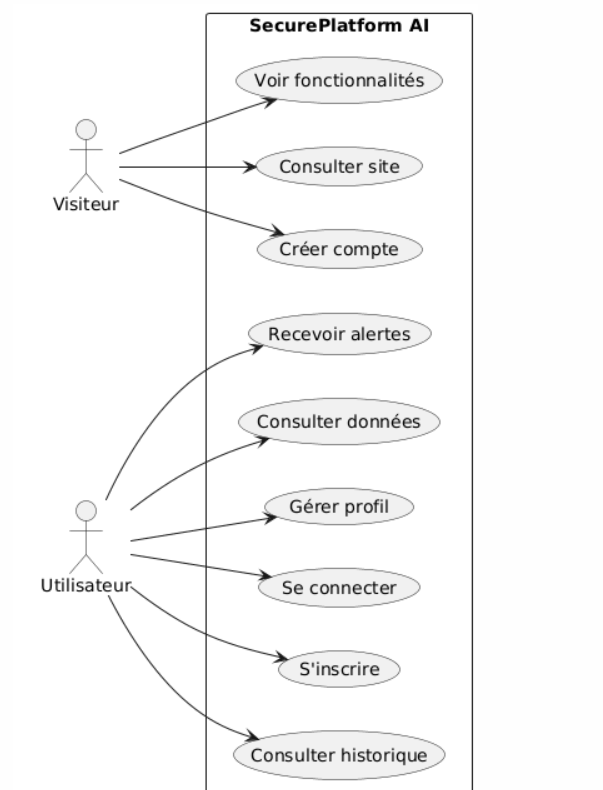
\includegraphics[width=0.9\textwidth]{UC1.png}
\caption{Diagramme de cas d'utilisation -- Visiteur}
\label{fig:usecase-visiteur}
\end{figure}

\section{Diagramme de cas d'utilisation -- Utilisateur}
\begin{figure}[H]
\centering
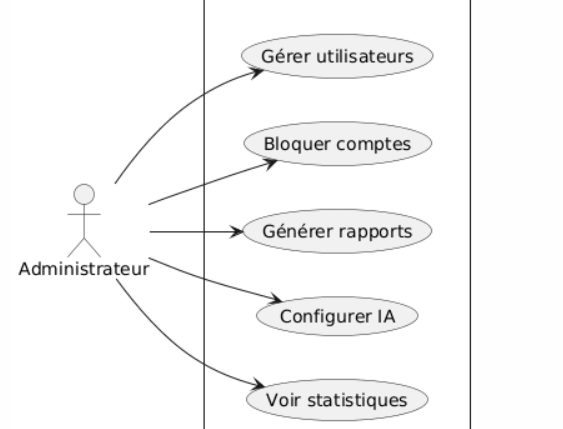
\includegraphics[width=0.9\textwidth]{UC2.png}
\caption{Diagramme de cas d'utilisation -- Utilisateur}
\label{fig:usecase-utilisateur}
\end{figure}

\section{Diagramme de cas d'utilisation -- Administrateur}
\begin{figure}[H]
\centering
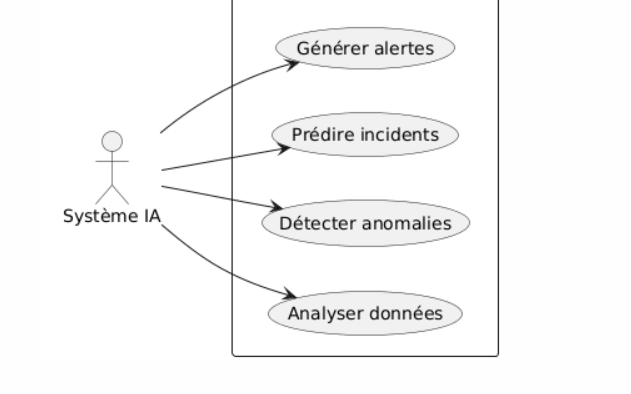
\includegraphics[width=0.9\textwidth]{UC3.png}
\caption{Diagramme de cas d'utilisation -- Administrateur}
\label{fig:usecase-admin}
\end{figure}

% ==========================
\chapter{Gestion de projet SCRUM}

\section{Backlog du produit (Product Backlog)}
Le backlog reprend les EPIC, Stories et Tasks et sert de base pour la méthodologie SCRUM.

\begin{longtable}{|p{3.5cm}|p{3.5cm}|p{9cm}|}
\hline
\textbf{EPIC} & \textbf{Story} & \textbf{Task} \\
\hline
\endfirsthead

\hline
\textbf{EPIC} & \textbf{Story} & \textbf{Task} \\
\hline
\endhead

\hline
\endfoot

\textbf{E1 — Cadrage \& Architecture} & E1-S1 — Définir le périmètre MVP & Lister fonctionnalités MVP in-scope (Stripe only, sans APIs opérateurs) \\
& & Lister out-of-scope (intégrations CNAM/STEG/Orange réelles) \\
& & Valider user stories prioritaires (User + Admin) \\
& E1-S2 — Finaliser architecture backend & Valider services finaux (Gateway, Auth, User, Wallet, Payment, Security, Notification, AI Risk, Reporting) \\
& & Définir communication Sync/Async \\
& & Définir topics Kafka v1 \\
\hline
\textbf{E2 — Setup Projet \& DevOps} & E2-S1 — Initialiser repos et standards & Créer structure mono-repo ou multi-repo \\
& & Ajouter conventions branches (main/dev/feature/*) \\
& & Ajouter templates PR + règles review \\
& E2-S2 — Environnement local & Docker Compose (PostgreSQL, Redis, Kafka, Grafana, Loki) \\
& & Ajouter health checks de chaque service \\
& & Documenter README démarrage local \\
& E2-S3 — CI/CD basique & Pipeline build + test unitaire \\
& & Scan qualité (lint + format) \\
& & Artifacts Docker images \\
\hline
\textbf{E3 — Auth \& User} & E3-S1 — Auth JWT & Endpoint register/login \\
& & Refresh token + logout \\
& & Middleware RBAC (User, Admin) \\
& E3-S2 — Profil utilisateur & CRUD profil \\
& & Préférences utilisateur (langue, notif) \\
& & Journaliser actions sensibles \\
\hline
\textbf{E4 — Wallet \& Ledger} & E4-S1 — Gestion wallet & Créer wallet à l'inscription \\
& & Endpoint consultation solde \\
& & Ledger immuable (credit/debit) \\
& E4-S2 — Historique wallet & Endpoint historique mouvements \\
& & Filtre date/statut/type \\
& & Pagination + tri \\
\hline
\textbf{E5 — Paiement Stripe} & E5-S1 — Checkout Stripe & Endpoint create-checkout-session \\
& & Mapper serviceType statique + montant \\
& & Sauvegarder transaction PENDING \\
& E5-S2 — Webhook Stripe & Vérifier signature webhook \\
& & Mettre transaction SUCCESS/FAILED \\
& & Publier événement Kafka paiement \\
& E5-S3 — Réconciliation basique & Idempotency key anti double paiement \\
& & Retry sécurisé en cas d'échec interne \\
& & Rapport journalier paiements \\
\hline
\textbf{E6 — Security Service} & E6-S1 — Collecte logs sécurité & Capturer login success/failed, IP, user-agent \\
& & Stocker security\_events \\
& & Ajouter correlation\_id partout \\
& E6-S2 — Règles temps réel & Rate-limit Redis \\
& & Blocklist IP (manual + auto rules) \\
& & Détection patterns SQLi basiques \\
& E6-S3 — Audit immuable & Table append-only admin actions \\
& & Chaînage hash (prev\_hash, curr\_hash) \\
& & Endpoint timeline sécurité admin \\
\hline
\textbf{E7 — Asynchrone Kafka (fiabilité)} & E7-S1 — Outbox pattern & Table outbox\_events \\
& & Worker de publication Kafka \\
& & Marquage PENDING/SENT/FAILED \\
& E7-S2 — Consumers robustes & Idempotent consumer via event\_id \\
& & Retry policy \\
& & Dead-letter topic (DLT) \\
\hline
\textbf{E8 — Notification Service} & E8-S1 — Notifications transactionnelles & Template email paiement réussi \\
& & Template email paiement échoué \\
& & Consommation événement payment.* \\
& E8-S2 — Fiabilité envoi & Retry envoi + backoff \\
& & Statuts sent/failed \\
& & Journal notifications \\
\hline
\textbf{E9 — AI Risk Service (Async)} & E9-S1 — Scoring risque & Consommer security.event.created \\
& & Calcul score (règles + modèle) \\
& & Publier risk.score.computed \\
& E9-S2 — Intégration Security & Action policy ALLOW/CHALLENGE/TEMP\_BLOCK \\
& & Alertes admin sur seuil critique \\
& & Fallback si IA down (règles only) \\
\hline
\textbf{E10 — Reporting \& Monitoring} & E10-S1 — Reporting métier & Agrégats paiements (jour/semaine/mois) \\
& & KPIs wallet (volume, succès, échecs) \\
& & Endpoint dashboard admin \\
& E10-S2 — Observabilité & Metrics Prometheus par service \\
& & Dashboards Grafana (paiement, sécurité, infra) \\
& & Logs centralisés Loki \\
\hline
\textbf{E11 — Tests \& Hardening} & E11-S1 — Tests & Unit tests services critiques \\
& & Integration tests (Stripe webhook flow) \\
& & E2E tests (login → paiement → notif) \\
& E11-S2 — Sécurité production & CORS strict + headers sécurité \\
& & Secrets management \\
& & Vérification conformité logs (pas de PII sensible) \\
\hline
\caption{Product Backlog}
\end{longtable}

\section{Planification des Sprints / Releases}
\begin{table}[H]
\centering
\begin{tabular}{|p{2cm}|p{2cm}|p{7cm}|p{4cm}|}
\hline
\textbf{Sprint} & \textbf{Durée} & \textbf{Contenu principal} & \textbf{Objectif Release} \\
\hline
Sprint 1 & 2 semaines & Setup projet + Auth + DB + Wallet de base & MVP minimum pour login + wallet \\
\hline
Sprint 2 & 2 semaines & Dashboard utilisateur + Profil + Historique wallet & MVP avec dashboard et gestion utilisateurs \\
\hline
Sprint 3 & 2 semaines & Paiement Stripe + Notification + Ledger complet & MVP complet pour transactions + notifications \\
\hline
Sprint 4 & 2 semaines & Security service + AI Risk service + Monitoring & Release 1 avec sécurité et scoring IA \\
\hline
Sprint 5 & 2 semaines & Reporting + tests finaux + hardening & Release finale prête production \\
\hline
\end{tabular}
\caption{Planification des Sprints / Releases}
\end{table}

\section{Répartition des rôles SCRUM}
\begin{table}[H]
\centering
\begin{tabular}{|p{4cm}|p{9cm}|}
\hline
\textbf{Rôle} & \textbf{Nom / Fonction} \\
\hline
Product Owner (PO) & AMOR Houssem -- responsable des exigences et priorités \\
Scrum Master (SM) & KHEDHIRI Montaha -- organisation, sprint planning, daily stand-up \\
Développeur Backend & BEN SLIMA Wissem -- API .NET 8, microservices, base de données \\
Développeur Frontend & BAHROUNI Seif -- Angular UI, dashboard utilisateur et admin \\
Développeur IA & AMOR Houssem -- modèle IA, scoring de risque, intégration Kafka \\
DevOps / QA & BEN SLIMA Wissem -- CI/CD, Docker, monitoring, tests \\
\hline
\end{tabular}
\caption{Rôles SCRUM}
\end{table}

\section{Choix Technologiques et Outils de Collaboration}
\begin{itemize}[leftmargin=*,label=--]
\item \textbf{Frontend :} Angular (TypeScript)
\item \textbf{Backend :} .NET 8 (C\#, architecture microservices)
\item \textbf{Base de données :} PostgreSQL (utilisateurs, transactions, logs), Redis (cache, sessions, rate-limiting)
\item \textbf{Messagerie asynchrone :} Apache Kafka (communication inter-services, patron Outbox)
\item \textbf{IA / ML :} Ollama (Mistral 7B, LLaMA 3) pour le scoring de risque ; Isolation Forest et Autoencoders (scikit-learn, HuggingFace) pour la détection d'anomalies ; CodeLlama pour la détection d'injections SQL
\item \textbf{Cloud / Infra :} AWS (free tier) ; Docker + Kubernetes (orchestration, scaling) ; Grafana + Prometheus (monitoring) ; Loki (logs centralisés)
\item \textbf{Outils de collaboration :} GitHub (versioning, PR, CI/CD via GitHub Actions) ; Jira (gestion des sprints et backlog)
\end{itemize}

\section{Développement du Sprint 1 (MVP)}

\subsection{Objectif Sprint 1}
Mise en place du projet + base de données + authentification + wallet minimal.

\subsection{Tâches Sprint 1}
\begin{table}[H]
\centering
\begin{tabular}{|p{6cm}|p{3cm}|p{2cm}|}
\hline
\textbf{Tâche} & \textbf{Responsable} & \textbf{Statut} \\
\hline
Initialiser repos Git + branches & Dev 1 & $\square$ \\
Config Docker Compose (PostgreSQL + Redis + Kafka) & DevOps & $\square$ \\
Endpoint register/login JWT + middleware RBAC & Dev Backend & $\square$ \\
Création wallet à l'inscription & Dev Backend & $\square$ \\
Endpoint consultation solde wallet & Dev Backend & $\square$ \\
Health checks services & DevOps & $\square$ \\
README + documentation setup local & DevOps & $\square$ \\
\hline
\end{tabular}
\caption{Tâches Sprint 1}
\end{table}

\subsection{Livrables Sprint 1}
\begin{itemize}[leftmargin=*,label=--]
\item Repo GitHub structuré
\item Base de données opérationnelle
\item Authentification JWT fonctionnelle
\item Wallet minimal fonctionnel
\item Documentation pour démarrage local
\end{itemize}

% ==========================
% Conclusion Générale (non numérotée)
% ==========================
\chapter*{Conclusion Générale}
\addcontentsline{toc}{chapter}{Conclusion Générale}

Ce rapport a présenté le projet \textbf{SaveSafe Wallet (SSW)}, une plateforme bancaire web sécurisée intégrant un portefeuille numérique et un système de détection de menaces par Intelligence Artificielle.

Nous avons détaillé le contexte et les objectifs du projet, la description fonctionnelle de la plateforme (gestion de comptes, wallet, paiements Stripe, sécurité IA, notifications, reporting), ainsi que l'étude comparative avec les solutions existantes sur le marché. La spécification des besoins fonctionnels et non fonctionnels a permis de cadrer précisément le périmètre du MVP, et l'identification des acteurs a clarifié les interactions attendues avec le système.

La méthodologie SCRUM a été adoptée avec un découpage en cinq sprints de deux semaines. Le product backlog couvre onze EPICs allant du cadrage initial jusqu'aux tests et au hardening de production. Le premier sprint, axé sur le setup projet, l'authentification JWT et le wallet minimal, constitue la base sur laquelle les sprints suivants viendront ajouter les modules de paiement, de sécurité IA, de notification et de reporting.

Les choix technologiques -- .NET 8 pour le backend, Angular pour le frontend, PostgreSQL et Redis pour les données, Apache Kafka pour la messagerie, et Ollama pour les modèles IA -- garantissent une architecture modulaire, performante et entièrement basée sur des outils open-source.

Les prochaines étapes consisteront à développer les sprints 2 à 5, intégrer les diagrammes d'architecture et de séquence détaillés, et préparer la release de production avec les tests E2E et le hardening sécurité.

\end{document}